%%%%%%%%%%%%%%%%%%%%%%%%%%%%%%%%%%%%%%%%%%%%%%%%%%%%%%%%%%%%%%%%%%%%%%
% How to use writeLaTeX: 
%
% You edit the source code here on the left, and the preview on the
% right shows you the result within a few seconds.
%
% Bookmark this page and share the URL with your co-authors. They can
% edit at the same time!
%
% You can upload figures, bibliographies, custom classes and
% styles using the files menu.
%
% If you're new to LaTeX, the wikibook is a great place to start:
% http://en.wikibooks.org/wiki/LaTeX
%
%%%%%%%%%%%%%%%%%%%%%%%%%%%%%%%%%%%%%%%%%%%%%%%%%%%%%%%%%%%%%%%%%%%%%%
\documentclass[a4paper, justified, notoc]{tufte-handout} % SZA: remove 'notoc' to regain tufte-style TOC

%\geometry{showframe}% for debugging purposes -- displays the margins

\usepackage{amsmath}

% Set up the images/graphics package
\usepackage{graphicx}
\setkeys{Gin}{width=\linewidth,totalheight=\textheight,keepaspectratio}
\graphicspath{{figures/}}

\title{How modern Web Browsers work\thanks{Special Topic for the Module ``Entwicklung Webbasierter Anwendungen''}}
\author[opt Author]{Prof.\ Dr.\ Stefan Zander}
\date{07.\ March 2018}  % if the \date{} command is left out, the current date will be used

% The following package makes prettier tables.  We're all about the bling!
\usepackage{booktabs}

% The units package provides nice, non-stacked fractions and better spacing
% for units.
\usepackage{units}

% The fancyvrb package lets us customize the formatting of verbatim
% environments.  We use a slightly smaller font.
\usepackage{fancyvrb}[baw]
\fvset{fontsize=\normalsize}

% SZA: Added to use a space between paragraphs
\setlength{\parskip}{0.5em}

% Small sections of multiple columns
\usepackage{multicol}

% Provides paragraphs of dummy text
\usepackage{lipsum}

% These commands are used to pretty-print LaTeX commands
\newcommand{\doccmd}[1]{\texttt{\textbackslash#1}}% command name -- adds backslash automatically
\newcommand{\docopt}[1]{\ensuremath{\langle}\textrm{\textit{#1}}\ensuremath{\rangle}}% optional command argument
\newcommand{\docarg}[1]{\textrm{\textit{#1}}}% (required) command argument
\newenvironment{docspec}{\begin{quote}\noindent}{\end{quote}}% command specification environment
\newcommand{\docenv}[1]{\textsf{#1}}% environment name
\newcommand{\docpkg}[1]{\texttt{#1}}% package name
\newcommand{\doccls}[1]{\texttt{#1}}% document class name
\newcommand{\docclsopt}[1]{\texttt{#1}}% document class option name

% SZA: Allows colored boxes
\usepackage[framemethod=tikz]{mdframed}

\usepackage[utf8]{inputenc} % this is needed for umlauts
% \usepackage[ngerman]{babel} % this is needed for umlauts
\usepackage[T1]{fontenc}    % this is needed for correct output of umlauts in pdf



% SZA: Added to provide learning objectives section
\newenvironment{lernziele}{
	\begin{mdframed}[hidealllines=true,backgroundcolor=gray!20] 
	\small \itshape
	\noindent \underline{Objectives:} 
	} 
	{ 
	\end{mdframed}
}

% SZA: The note commands extends the marginnote with additional text
\newcommand{\note}[1] {
	\marginnote{\textbf{Note:}\quad #1 } }


% SZA: Added to support JavaScript in LaTeX Code
%Define the listing package
\usepackage{listings} %code highlighter
\usepackage{color} %use color
\definecolor{mygreen}{rgb}{0,0.6,0}
\definecolor{mygray}{rgb}{0.5,0.5,0.5}
\definecolor{mymauve}{rgb}{0.58,0,0.82}

 
%Customize a bit the look
\lstset{ %
backgroundcolor=\color{gray!20}, % choose the background color; you must add \usepackage{color} or \usepackage{xcolor}
basicstyle=\small, % the size of the fonts that are used for the code
breakatwhitespace=false, % sets if automatic breaks should only happen at whitespace
breaklines=true, % sets automatic line breaking
captionpos=b, % sets the caption-position to bottom
commentstyle=\color{mygreen}, % comment style
deletekeywords={...}, % if you want to delete keywords from the given language
escapeinside={\%*}{*)}, % if you want to add LaTeX within your code
extendedchars=true, % lets you use non-ASCII characters; for 8-bits encodings only, does not work with UTF-8
frame=single, % adds a frame around the code
keepspaces=true, % keeps spaces in text, useful for keeping indentation of code (possibly needs columns=flexible)
keywordstyle=\color{blue}, % keyword style
% language=Octave, % the language of the code
morekeywords={*,...}, % if you want to add more keywords to the set
numbers=left, % where to put the line-numbers; possible values are (none, left, right)
numbersep=5pt, % how far the line-numbers are from the code
numberstyle=\large\color{black}, % the style that is used for the line-numbers
rulecolor=\color{black}, % if not set, the frame-color may be changed on line-breaks within not-black text (e.g. comments (green here))
showspaces=false, % show spaces everywhere adding particular underscores; it overrides 'showstringspaces'
showstringspaces=false, % underline spaces within strings only
showtabs=false, % show tabs within strings adding particular underscores
stepnumber=1, % the step between two line-numbers. If it's 1, each line will be numbered
stringstyle=\color{mymauve}, % string literal style
tabsize=2, % sets default tabsize to 2 spaces
title=\lstname % show the filename of files included with \lstinputlisting; also try caption instead of title
}
%END of listing package%
 
\definecolor{darkgray}{rgb}{.4,.4,.4}
\definecolor{purple}{rgb}{0.65, 0.12, 0.82}
\definecolor{darkgreen}{rgb}{.0,.5,.0}

 
%define Javascript language
\lstdefinelanguage{JavaScript}{
keywords={typeof, new, true, false, catch, function, return, null, catch, switch, var, if, in, while, do, else, case, break},
keywordstyle=\color{orange}\bfseries,
ndkeywords={class, export, boolean, throw, implements, import, this},
ndkeywordstyle=\color{darkgray}\bfseries,
identifierstyle=\color{black},
sensitive=false,
comment=[l]{//},
morecomment=[s]{/*}{*/},
commentstyle=\color{darkgray}\ttfamily,
stringstyle=\color{blue}\ttfamily,
morestring=[b]',
morestring=[b]"
}
 
\lstset{
language=JavaScript,
extendedchars=true,
basicstyle=\small\ttfamily,
showstringspaces=false,
showspaces=false,
numbers=left,
numberstyle=\tiny,
numbersep=9pt,
tabsize=2,
breaklines=true,
showtabs=true,
captionpos=b,
frame=l % was 'l' || was lines
}


% SZA: Print listing captions to the right margin to better accomodate the tufte style
% from: https://tex.stackexchange.com/questions/282485/use-listings-in-tufte-book-with-captions-in-margin
\makeatletter
% textwidth Tuftian float for listings
\newenvironment{listing}[1][htbp]
  {\ifvmode\else\unskip\fi\begin{@tufte@float}[#1]{lstlisting}{}}
  {\end{@tufte@float} } % SZA: Added \vspace{-2em} \vspace command in order to better align the following paragraph
% fullwidth Tuftian float for listings
\newenvironment{listing*}[1][htbp]%
  {\ifvmode\else\unskip\fi\begin{@tufte@float}[#1]{lstlisting}{star}}
  {\end{@tufte@float}}
% enable re-use of \listoflistings facility
\def\ext@lstlisting{lol}
% show listing number in caption even though \lst@@caption is empty
\def\fnum@lstlisting{\lstlistingname~\thelstlisting}
\makeatother





\begin{document}
\maketitle% this prints the handout title, author, and date

% \begin{abstract}
% \noindent Lernziele:
% \begin{itemize}
% 	\item Kennenlernen der Grundtechniken moderner HTML5 Echtzeitanwendungen
% 	\item Aufbau des WebSocket Protokolls
% 	\item Entwicklung erster WebSocket-basierter Client-Server-Anwendungen
% 	\item Entwicklung einfacher WebSocket-Server mittels JavaScript und dem Vert.x Framework
% \end{itemize}
% \end{abstract}

\begin{lernziele}
\begin{itemize}
	% \item Learn about the processing internals of modern Web browsers
	\item Learn about the basic building blocks of modern Web browsers 
	\item Get acquainted with the processing internals and the DOM building logic
	\item Understand what happens inside the browser when you type in an URL
\end{itemize}
\end{lernziele}

%\printclassoptions

\setcounter{secnumdepth}{2} % SZA: Added to have numbers in sections

\noindent \rule{1.54\textwidth}{0.4pt}
\tableofcontents
\noindent \rule{1.54\textwidth}{0.4pt}



\section{Preface} % (fold)
\label{sec:preface}
\marginnote[-3em]{This lecture note is a revised summary of the excellent article ``How Browsers Work: Behind the scenes of modern web browsers'' published by Tali Garsiel and Paul Irish in 2011. The original article is available at: \url{https://www.html5rocks.com/en/tutorials/internals/howbrowserswork/}. 

\vspace{1em} 
There is also a video available at vimeo about Tali's talk: \url{http://vimeo.com/44182484}.}

\begin{quote}
	\emph{In the years of IE 90\% dominance there was nothing much to do but regard the browser as a ``black box'', but now, with open source browsers having more than half of the usage share, it's a good time to take a peek under the engine's hood and see what's inside a web browser. Well, what's inside are millions of C++ lines...}\begin{flushright}\vspace{-1em}---Tali Garsiel \end{flushright}
\end{quote}

The following information and facts about the internal operation principles of WebKit and Gecko is the result of extensive research done by the Israeli developer \textbf{Tali Garsiel}. Over a few years, she reviewed all the published data about browser internals and spent a lot of time reading Web browser source code. Tali published her research on her site\sidenote{See \url{http://taligarsiel.com/}}. In the following years, her research results have been revised and republished on numerous occasions and provided insights to a larger audience. 

\textbf{Why should you learn about browser internals?}

Learning the internals of browser operations helps you make better decisions and know the justifications behind development best practices. It also helps you to identify performance bottlenecks and build lightning fast websites. As we will see\marginnote{TODO: Add refs}, page loading time has an influence on the Google page rank---a page loading time > 2 sec.\ results in a lower rank in the Google search results and the Google crawler also crawls such pages less frequently, meaning that  search index terms are less frequently updated and the time until new or updated page content will be considered by the Google search engine is extended.   







% section preface (end)



\section{Introduction}\label{sec:introduction}
\begin{quote}
	\emph{``I just had to take the hypertext idea and connect it to the TCP and DNS ideas and—ta-da!—the World Wide Web.''\sidenote{One of the famous quotes Sir Tim Berners-Lee used to say about the development of the World Wide Web... \citep{history:2018}}}\begin{flushright}\vspace{-1em}---Sir Tim Berners-Lee, inventor of the World Wide Web \end{flushright}
\end{quote}



Web browsers are the most widely used software.
This lecture explains their fundamental operation principles so that students get an understanding about the things that happen internally when a website is requested, i.e., the time from typing in a website's URL in the browser's address bar until it is rendered by in the browser's viewport.

The complexity of Web browser software has significantly changed over recent years---as the following two screenshots indicate:

\begin{figure}%
	\centering
  \includegraphics[width=1.0\textwidth]{./figures/lynx_browser.png}
  \caption[][0em]{Screenshot of the Lynx Browser, the first and purely text-based browser for the World Wide Web.}
  \label{fig:lynx}
\end{figure}

\begin{figure}%
	\centering
  \includegraphics[width=1.0\textwidth]{./figures/next_browser.png}
  \caption[][0em]{Screenshot of the first WWW browser with a graphical user interface, the NeXT Browser used at CERN.}
  \label{fig:next_browser}
\end{figure}

TODO: Add image of first NEXT browser; compare it with inspector of Google Chrome; add some description (refs are in the keynote file)


\subsection{What is a Web Browser}
\label{sub:what_is_a_web_browser}
\marginnote[-2em]{See \url{https://seng130.wordpress.com/lectures-2/browser-architecture/}}


This section outlines some of the central functionalities provided by a modern Web browser. It helps in understanding what a browser exactly is. 

\begin{enumerate}
	\item Is an application that we use when we browse the World Wide Web.
	\item It renders text-based HTML documents into visual pages, which are what we see inside a browser.
	\item It speaks HTTP protocol and communicates with Web servers.
	\item It understands URL and knows how to translates URL into Web resources, e.g., HTML text files, images, videos, etc. (\emph{URL dereferencing})
	\item It is a virtual machine that runs the JavaScript programs embedded inside HTML documents.
	\item It understands CSS rules and applies the rules to layout the pages.
	\item It interacts with a user in front of a browser and translates user inputs into browser events, e.g., clicking a link, clicking a button, submitting text inside a text box.
	% \item It makes the WWW come alive!
	\item It provides sophisticated tools for analyzing the structure of Web content and network traffic 
	\item It contains a JavaScript console to utilize its JavaScript engine 
\end{enumerate}





\section{The Browser's Main Functionality} % (fold)
\label{sec:the_browser_s_main_functionality}
The main function of a browser is to present the web resource you choose, by requesting it from the server and displaying it in the browser window. The resource is usually an HTML document, but may also be a PDF, image, or some other type of content. The location of the resource is specified by the user using a URI (Uniform Resource Identifier).

The way the browser interprets and displays HTML files is specified in the HTML and CSS specifications. These specifications are maintained by the \textbf{World Wide Web Consortium} organization\sidenote{\url{https://www.w3.org/}}, commonly denominated as \textbf{W3C}, which is the standards organization for the web. For years browsers conformed to only a part of the specifications and developed their own extensions. That caused serious compatibility issues for web authors. Today most of the browsers more or less conform to the specifications.

Browser user interfaces have a lot in common with each other. Among the common user interface elements are:
\begin{itemize}
	\item Address bar for inserting a URI
	\item Back and forward buttons
	\item Bookmarking options
	\item Refresh and stop buttons for refreshing or stopping the loading of current documents
	\item Home button that takes you to your home page
\end{itemize}

Strangely enough, the browser's user interface is \emph{not specified} in any formal specification, it just comes from good practices shaped over years of experience and by browsers imitating each other. The HTML5 specification does not define UI elements a browser must have, but lists some common elements. Among those are the address bar, status bar and tool bar. There are, of course, features unique to a specific browser like Firefox's downloads manager.


\section{The Browser's High Level Structure} % (fold)
\label{sub:the_browser_s_high_level_structure}

The\marginnote{A reference architecture for modern Web browsers} following components are considered the main building blocks of modern Web browsers (cf.~\citep{grosskurth:2006}):
\begin{enumerate}
	\item \textbf{The user interface}: this includes the address bar, back/forward button, bookmarking menu, etc. Every part of the browser display except the window where you see the requested page.
	\item \textbf{The browser engine}: marshals actions between the UI and the rendering engine.
	\item \textbf{The rendering engine}: responsible for displaying requested content. For example if the requested content is HTML, the rendering engine parses HTML and CSS, and displays the parsed content on the screen.
	\item \textbf{Networking}: Responsible for network calls such as HTTP requests, using different implementations for different platform behind a platform-independent interface.
	\item \textbf{UI backend}: used for drawing basic widgets like combo boxes and windows. This backend exposes a generic interface that is not platform specific. Underneath it uses operating system user interface methods.
	\item \textbf{JavaScript interpreter}: Used to parse and execute JavaScript code.
	\item \textbf{Data storage}: This is a persistence layer. The browser may need to save all sorts of data locally, such as cookies. Browsers also support storage mechanisms such as localStorage, IndexedDB, WebSQL and FileSystem.
\end{enumerate}

Figure~\ref{fig:reference_architecture} provides a graphical overview of the reference elements together with a visualization of their relationships among each other. Figure~\ref{fig:mozilla_architecture} shows an implementation of the reference architecture elements for the Firefox browser.


\begin{figure}%
	\centering
  \includegraphics[width=0.9\textwidth]{./figures/browser_reference_architecture.png}
  \caption[][0em]{A reference architecture for Web browsers~\citep{grosskurth:2006}}
  \label{fig:reference_architecture}
\end{figure}

\begin{figure}%
	\centering
  \includegraphics[width=1.0\textwidth]{./figures/mozilla_browser_architecture.png}
  \caption[][0em]{The Firefox browser architecture is based upon the reference architecture components~\citep{grosskurth:2006}}
  \label{fig:mozilla_architecture}
\end{figure}

It is important to note that browsers such as Chrome run multiple instances of the rendering engine: one for each tab. Each tab runs in a separate process.

\subsection{The Rendering Engine} % (fold)
\label{sub:the_rendering_engine}
Different browsers use different rendering engines: Internet Explorer uses Trident, Firefox uses Gecko, Safari uses WebKit. Chrome and Opera (from version 15) use Blink, a fork of WebKit.

WebKit is an open source rendering engine which started as an engine for the Linux platform and was modified by Apple to support Mac and Windows. See \url{webkit.org} for more details.

By default the rendering engine can display HTML and XML documents and images. It can display other types of data via plug-ins or extension; for example, displaying PDF documents using a PDF viewer plug-in. However, in this chapter we will focus on the main use case: displaying HTML and images that are formatted using CSS.

\paragraph{Workflow}

\begin{figure}%
	\centering
  \includegraphics[width=1.0\textwidth]{./figures/webkit_main_flow.png}
  \caption[][0em]{The default workflow of the WebKit render engine}
  \label{fig:webkit_main_flow}
\end{figure}

The rendering engine will start parsing the HTML document and convert elements to DOM nodes in a tree called the \textbf{content tree}. The engine will parse the style data, both in external CSS files and in style elements. Styling information together with visual instructions in the HTML will be used to create another tree: the \textbf{render tree}.

The render tree contains rectangles with visual attributes like color and dimensions. The rectangles are in the right order to be displayed on the screen.

After the construction of the render tree it goes through a \textbf{layout process}. This means giving each node the exact coordinates where it should appear on the screen. The next stage is painting---the render tree will be traversed and each node will be painted using the UI backend layer.

It is important to understand that this is a \emph{gradual process}. For better user experience, the rendering engine will try to display contents on the screen as soon as possible\sidenote{This is referred to as the \textbf{Compositing Forest} (cf.\ \url{https://www.chromium.org/developers/design-documents/gpu-accelerated-compositing-in-chrome}) since four conceptually different tree structures are processed in parallel (DOM tree, RenderObject tree, RenderLayer tree, GraphicsLayer tree).}. It will not wait until all HTML is parsed before starting to build and layout the render tree. Parts of the content will be parsed and displayed, while the process continues with the rest of the contents that keeps coming from the network.

\paragraph{Parsing} % (fold)
\label{par:parsing}
Since parsing is a very significant process within the rendering engine, we will go into it a little more deeply. Let's begin with a little introduction about parsing.

Parsing\marginnote{Parsing is based on the syntax rules the document obeys: the language or format it was written in. Every format you can parse must have deterministic grammar consisting of vocabulary and syntax rules. It is called a context free grammar. Human languages are not such languages and therefore cannot be parsed with conventional parsing techniques.} a document means translating it to a structure the code can use. The result of parsing is usually a tree of nodes that represent the structure of the document. This is called a parse tree or a syntax tree.

Parsing can be separated into two sub processes: \textbf{lexical analysis} and \textbf{syntax analysis}.

\textbf{Lexical analysis} is the process of breaking the input into tokens. Tokens are the language vocabulary: the collection of valid building blocks. In human language it will consist of all the words that appear in the dictionary for that language.

\textbf{Syntax analysis} is the applying of the language syntax rules.

The parsing process is \textbf{iterative}. The parser will usually ask the lexer\sidenote{The lexer (sometimes called \emph{tokenizer}) that is responsible for breaking the input into valid tokens.} for a new token and try to match the token with one of the syntax rules. If a rule is matched, a node corresponding to the token will be added to the parse tree and the parser will ask for another token.

If no rule matches, the parser will store the token internally, and keep asking for tokens until a rule matching all the internally stored tokens is found. If no rule is found then the parser will raise an exception. This means the document was not valid and contained syntax errors.

\subsection{HTML Content Parsing} % (fold)
\label{sub:parsing_html_content}

There are programs that can create parsers for languages that are defined on the bases of a context free grammar. 
Such grammars can usually described using the Backus Naur Form (BNF).
However, human language and HTML (as we will see) are not context free grammars. 
Therefore, a standard parser for parsing HTML does not exist. 
This has some consequence for Web development:







% Die Ladezeit einer Webseite ist eines wenn nicht das wichtigste Kriterium einer guten Web Usability. Eine Ladezeit von < 1 Sekunde wird als Heiliger Gral angesehen, nach dem alle News-Sites, Onlineshops, Portale, Blogs und Landingpages suchen. Denn an der Ladezeit hängen sowohl Nutzerzufriedenheit als auch Konversionsraten und deshalb letztlich Traffic und Umsatz einer Seite. Der Einfluss ist so immens, dass beispielsweise Amazon bei einem Anstieg der Ladezeit um 0,1 Sekunden bereits ein Prozent an Umsatz verlieren würde~\citep{heise:2018}.
%
% Das Problem besteht insbesondere auch bei mobilen Webseiten, wie nachfolgendes Zitat verdeutlicht~\citep{hobo:2018}:
% \begin{quote}
% 	\emph{``The average time it takes to fully load a mobile landing page is 22 seconds, according to a new analysis. \textbf{Yet 53\% of visits are abandoned if a mobile site takes longer than three seconds to load.} That’s a big problem.''}\begin{flushright}\vspace{-1em}---Google \end{flushright}
% \end{quote}
%
% Google Research hat hierzu interessante Studien veröffentlich~\citep{an:2016}:
% \begin{quote}
% 	\emph{``Mobile sites lag behind desktop sites in key engagement metrics such as average time on site, pages per visit, and bounce rate. For retailers, this can be especially costly since 30\% of all online shopping purchases now happen on mobile phones. The average U.S. retail mobile site loaded in 6.9 seconds in July 2016, but, according to the most recent data, \textbf{40\% of consumers will leave a page that takes longer than three seconds to load}. And \textbf{79\% of shoppers who are dissatisfied with site performance} say they're less likely to purchase from the same site again.''}
% \end{quote}
%
% Mit Hilfe eines neuronalen Netzwerks fand man heraus, dass die Hauptfaktoren, die sich für die Dauer des Seitenaufbaus verantwortlich zeichnen die \begin{itemize}
% 	\item Anzahl der Seitenelemente, sowie
% 	\item die Anzahl der enthaltenen Bilder
% \end{itemize} sind. Bei komplexen Seiten mit vielen Elementen dauert das Parsen des Seitencodes sowie der Aufbau des DOMs bedeutend länger. Bei Grafiken sollte man auflösungsoptimierte JPEGs anstatt PNG Formate verwenden.
%
% Eine weitere Studie, welche die \textbf{Bounce rate}\marginnote{Die \emph{Bounce rate} misst den prozentualen Anteil der Nutzer, die eine Web-Präsenz nach der Startseite wieder verlassen ohne die weiteren Inhalte in Augenschein genommen zu haben (\emph{``[...]without exploring beyond the landing page.''}). } -- also das Verlassen einer Seite ohne deren Inhalt genauer in Augenschein zu nehmen -- untersucht hat, kommt zu folgendem Ergebnis~\citep{google:2017}:
%
% \begin{quote}
% 	\emph{``Recently, we trained a deep neural network—a computer system modeled on the human brain and nervous system—with a large set of bounce rate and conversions data. The neural net, which had a 90\% prediction accuracy, found that as page load time goes from one second to seven seconds, the probability of a \textbf{mobile site visitor bouncing increases 113\%}. Similarly, as the number of elements—text, titles, images—on a page goes from 400 to 6,000, the \textbf{probability of conversion drops 95\%}.''}
% \end{quote}
%
% Weitere Interessante Einblicke einschließlich Maßnahmen zur Behebung von Geschwindigkeitsproblemen bietet die folgende Seite\sidenote{\url{https://www.thinkwithgoogle.com/marketing-resources/experience-design/mobile-page-speed-load-time/}}.
%
% Aufgrund solcher Ergebnisse ist es nicht verwunderlich, dass Unternehmen wie Google seit Jahren das Thema Webperformance vorantreiben und sich die \textbf{Ladezeit einer Seite sogar auf ihre Platzierung in den Google-Suchergebnissen auswirkt}.
%
% Technisch gesehen hängt die Ladezeit einer Seite an drei zentralen Faktoren:
% \begin{enumerate}
% 	\item an der Verarbeitung im Server,
% 	\item an der Übertragung über das Netzwerk, und
% 	\item an der Darstellung im Browser.
% \end{enumerate}
% Alle drei können einen starken Einfluss auf die Performance haben und die Ladezeitoptimierung zu einem langen und komplexen Prozess machen.
%
% Einen dieser drei Aspekte -- die Übertragung der Webseite vom Server zum Browser -- konnten Entwickler bislang kaum beeinflussen. Seit 1999 ist das Hypertext Transfer Protocol HTTP in der Version 1.1 der Standard zur Datenübermittlung im Web\marginnote{Nur zur Erinnerung: im Jahre 1999 war der bedeutendste Hersteller für Mobiltelefone ein Unternehmen aus Finnland mit dem Namen Nokia. Der Präsident der USA hieß Bill Clinton. Apple lieferte seine Rechner mit fest verbauten Bildröhren aus, und deutsche Kunden bezahlten dafür damals nicht in Euro, sondern in D-Mark. Quelle:~\citep{weinschenkler:2017}}. Nach über 15 Jahren gibt es nun mit Version 2 (auch HTTP/2 oder kurz h2 genannt) den langersehnten Nachfolger.
%
%
%
%
% \section{HTTP/2} % (fold)
% \label{sec:http_2}
% HTTP/2 stellt den Nachfolger von HTTP/1.1 dar und basiert auf dem von Google entwickelten SPDY (Speedy) Protokoll\sidenote{SPDY Whitepaper des Chromium Projekts: \url{https://www.chromium.org/spdy/spdy-whitepaper}}. Im Gegensatz zu SPDY benötigt HTTP/2 keine Verschlüsselung mittels TLS (Transport Layer Security) und kann auch für HTTP Seiten verwendet werden~\citep{mueller:2015}. Langfristig soll HTTP/1.1 durch HTTP/2 abgelöst werden und sich als Standard etablieren. Vorerst stellt die neue Protokollversion jedoch nur eine Alternative dar und gewährleistet durch Abwärtskompatibilität, dass auch Browser, die dieses Protokoll nicht unterstützen, Webseiten über HTTP/1.1 laden.
%
% HTTP/2 ist ein Binärprotokoll, setzt einen klaren Fokus auf Performance und gibt Entwicklern verschiedene Möglichkeiten zur Optimierung der Seitenladezeit an die Hand.
% Version 2 des Hypertext Transfer Protokolls\sidenote{Spezifikation: \url{https://tools.ietf.org/html/rfc7540}} wurde im Mai 2015 von der Internet Engineering Task Force (IETF) als Standard verabschiedet.
% Ziel von HTTP/2 ist, die Bandbreite im World Wide Web besser auszunutzen und die Netzwerk-Latenz zu verringern. Hierzu beinhaltet HTTP/2 einige zentrale Optimierungen gegenüber HTTP/1.1, wie insbesondere \textbf{Request Multiplexing}, \textbf{Header Compression}, \textbf{Resource Prioritization}, und \textbf{Server Push}\sidenote{Siehe Kapitel~\ref{sub:semantik_und_bestandteile}}.
% Request Multiplexing und die Kompression der Headerinformationen verbessern die Ladezeit einer Seite unmittelbar. Um die anderen beiden Optimierungen zu nutzen, ist ein gewisser Entwicklungsaufwand erforderlich.
%
% \begin{figure}%
% 	\centering
%   \includegraphics[width=1.5\textwidth]{./figures/http2_demo_people.png}
%   \caption[][21em]{Vergleich der Ladezeiten zwischen HTTP/1.1 (linke Hälfte) und HTTP/2 (rechte Bildhälfte) am Beispiel einer aus vielen kleinen Bildschnipseln zusammengesetzten großen Bilddatei (Demo auf \url{http://www.http2demo.io/})}
%   \label{fig:http2_demo_1}
% \end{figure}
%
% \begin{figure}%
% 	\centering
%   \includegraphics[width=1.5\textwidth]{./figures/http2_demo_globe.png}
%   \caption[][26em]{Vergleich der Ladezeiten zwischen HTTP/1.1 (linke Hälfte) und HTTP/2 (rechte Bildhälfte) am Beispiel einer aus vielen kleinen Bildschnipseln zusammengesetzten großen Bilddatei (Demo auf \url{https://http2.akamai.com/demo})}
%   \label{fig:http2_demo_2}
% \end{figure}
%
% Abbildung~\ref{fig:http2_demo_1} und~\ref{fig:http2_demo_2}\marginnote{HTTP/2 Webdemos: \begin{itemize}
% 	\item \url{http://www.http2demo.io/}
% 	\item \url{https://http2.akamai.com/demo}
% \end{itemize} } zeigen die Ladezeiten einer großen Bilddatei, die sich aus vielen kleinen Bildschnippseln (\emph{sprites}) zusammensetzt. In der linken Bildhälfte ist jeweils  die Ladezeit mittels HTTP/1.1 zu sehen, die rechte Bildhälfte zeigt die Ladezeit mit dem HTTP/2 Protokoll. Sowohl das erste, als auch das zweite Beispiel zeigen eine deutliche Verbesserung der Ladezeiten unter HTTP/2.
% Zum selber testen finden sich die beiden Demos unter \url{http://www.http2demo.io/} sowie \url{https://http2.akamai.com/demo}.
%
%
%
%
%
%
%
% \subsection{Semantik und Bestandteile} % (fold)
% \label{sub:semantik_und_bestandteile}
% Die Semantik des HTTP-Protokolls bleibt mit Version 2 unberührt; die bekannten HTTP-Schlüsselwörter wie \texttt{GET}, \texttt{POST}, \texttt{PUT}, \texttt{DELETE} oder \texttt{OPTIONS} bleiben erhalten. Auf der Anwendungsschicht ändert sich nichts. Neu ist die Abwicklung des Transports der Header und Nutzdaten. HTTP-Requests und -Responses sind in \textbf{Streams}, \textbf{Messages} und \textbf{Frames} kodiert. Das HTTP/2-Protokoll besteht aus folgenden Bausteinen:
%
% \begin{itemize}
% 	\item \textbf{Stream}: Ein bidirektionaler Austausch von Daten zwischen Server und Client, der aus einer oder mehreren Messages besteht. Die Übertragung eines Streams erfolgt innerhalb einer TCP-Verbindung. Mehrere Streams lassen sich simultan über dieselbe TCP-Verbindung übertragen.
% 	\item \textbf{Message}: Eine komplette Abfolge von Frames, die zu einer logischen Message gehören. Eine Message gehört zu einem Stream.
% 	\item \textbf{Frame}: Die kleinste Kommunikationseinheit innerhalb von HTTP/2. Sie enthält binär kodierte Header- oder Nutzdaten.
% \end{itemize}
%
% Das Zusammenspiel dieser Bausteine kann wie folgt beschrieben werden:
% \begin{itemize}
% 	\item Die gesamte Kommunikation zwischen einem Client und dem Server wird über eine TCP-Verbindung abgehandelt, welche eine nahezu beliebige Anzahl an bidirektionalen Streams beinhalten kann.
% 	\item Jeder Stream besitzt einen eindeutigen Identifier und optionale Prioritätsinformationen
% 	\item Jede Message ist eine logische HTTP-Request oder Response Nachricht, welche aus einem oder mehreren Frames besteht.
% 	\item Ein Frame ist die kleinste Kommunikationseinheit über die Daten wie HTTP Header, Message Payload (Nachrichteninhalt) etc.\ transportiert werden.
% \end{itemize}
%
% Zusammengefasst unterteilt HTTP/2 die HTTP Protokollkommunikation in einen Austausch binär-kodierter Frames, welche Nachrichten zugeordnet sind die zu einem bestimmten Stream gehören.
%
% \begin{figure}%
% 	\centering
%   \includegraphics[width=1\textwidth]{./figures/http2_streams.png}
%   \caption{Beispielhafte Darstellung eines HTTP/2-Nachrichtenaustauschs zwischen Browser und Server~\citep{weinschenkler:2017}.}
%   \label{fig:http2_nachrichtenaustausch}
% \end{figure}
%
% Abbildung~\ref{fig:http2_nachrichtenaustausch} zeigt eine beispielhafte Client-Server-Kommunikation (übernommen von~\citep{weinschenkler:2017}). Der komplette Nachrichtenaustausch läuft über genau eine TCP-Verbindung ab. Die dabei versendeten sechs Frames werden in nachfolgender Auflistung erläutert:
%
% \begin{enumerate}
% 	\item Der Client beginnt, indem er einen Request für die Datei \texttt{index.html} per \texttt{HEADERS}-Frame an den Server schickt. Dafür eröffnet er einen neuen Stream -- einen in sich abgeschlossenen Nachrichtenaustausch mit dem Server --, der die \texttt{ID 41} erhält. Der Client setzt weiterhin zwei Flags in dem Frame. \texttt{+END\_HEADERS} bedeutet, dass der Client im aktuellen Stream keine weiteren \texttt{HEADERS}-Frames mehr versenden wird. \texttt{+END\_STREAM} bedeutet, dass der Client nicht beabsichtigt, weitere Frames im aktuellen Stream zu versenden.
% 	\item Der Server kann die Datei \texttt{index.html} ausliefern und schickt innerhalb desselben Streams \texttt{41} ebenfalls einen \texttt{HEADERS}-Frame mit dem Statuscode \texttt{200} an den Client zurück. Der Code ist bereits aus HTTP/1.1 bekannt und besagt, dass die Datei verfügbar ist und der Client sie demnächst erhalten wird. Neu ist, dass der Server die eigentliche Nutzlast in Form der Datei \texttt{index.html} mit einem separaten \texttt{DATA}-Frame verschickt.
% 	\item Der Server schickt einen \texttt{PUSH\_PROMISE}-Frame, eine Neuerung, mit der er von sich aus eine Datenübertragung an den Client initiiert. Im Fall des Beispiels von Abbildung~\ref{fig:http2_nachrichtenaustausch} antizipiert der Server, dass der Client direkt nach seinem Request für die Datei \texttt{index.html} die Datei \texttt{style.css} benötigen wird. Deshalb bietet er an, diese Datei über den neuen Stream \texttt{42} an den Client zu versenden.
% 	\item Wie bei Punkt 2 schickt der Server nun im Stream \texttt{42} einen \texttt{HEADERS}-Frame mit dem Statuscode \texttt{200} bezogen auf die Datei \texttt{style.css} an den Client. Letzterer kündigt die baldige Übertragung der Datei an. Ohne weiteren Widerspruch des Clients würde als nächstes im Stream \texttt{42} die Übertragung eines \texttt{DATA}-Frame mit der \texttt{style.css} erfolgen.
% 	\item Im Beispiel benötigt der Client die Datei \texttt{style.css} nicht, weil er noch eine Kopie davon in seinem Cache zur Verfügung hat. Er sendet deshalb im Stream \texttt{42} einen \texttt{RST\_STREAM}-Frame. Damit schließt er den Stream \texttt{42}, und der Server wird darüber keinerlei Daten mehr versenden.
% 	\item Bleibt noch die eingangs durch den Client im Stream \texttt{41} angefragte Datei \texttt{index.html}, die der Server nun in einem \texttt{DATA}-Frame an den Client versendet. Damit beendet der Server seinerseits die Kommunikation im Stream \texttt{41}.
% \end{enumerate}
%
%
%
% \subsection{Übersicht der Neuerungen} % (fold)
% \label{sub:neuerungen}
% % subsection neuerungen (end)
% Wie eingangs beschrieben nutzt HTTP/2 die bestehende Bandbreite bei der Datenübertragung besser aus als seine Vorgänger. Das erreicht der neue Standard durch vier Neuerungen.
% \begin{enumerate}
% 	\item \textbf{Request Multiplexing} \\ Das Request Multiplexing sorgt dafür, dass mehrere Request-/Response-Konversationen gleichzeitig über ein und dieselbe TCP-Verbindung erfolgen können.
% 	\item \textbf{Server Push} \\ Das Konzept des Server Push ermöglicht, dass ein HTTP-Client einen HTTP Request in Richtung Server absetzen und Letzterer darauf mit mehr als einer Response antworten kann.
% 	\item \textbf{Header Compression} \\ HTTP/2 verwendet eine verbesserte Implementierung zur Datenkompression speziell für die Protokoll-Metadaten -- den HTTP Header.
% 	\item \textbf{Resource Priorization} \\ Datenpakete werden nach Wichtigkeit sortiert und in entsprechender Reihenfolge übermittelt, wodurch zuerst die Dateien an den Browser übermittelt werden, die für einen schnellen Seitenaufbau wichtig sind (vgl.~\cite{mueller:2015}).
% \end{enumerate}
%
%
% Diese Vorlesungseinheit gibt einen Überblick über die zentralen Ideen und Techniken von HTTP/2 und setzt sie in Bezug zu anderen Techniken zur Steigerung der Webperformance.
%
% \subsection{Request Multiplexing} % (fold)
% \label{sub:reduktion_der_ladezeiten}
% HTTP/1.1\marginnote{HTTP/1.1 erlaubt jeweils nur eine Request-Response-Konversation pro TCP-Verbindung} bietet keine direkte Möglichkeit, Requests zu parallelisieren. Über eine TCP-Verbindung kann jeweils nur ein HTTP-Request und daraufhin nur eine HTTP-Response fließen. Das ist für zeitgemäße Webseiten problematisch. Die Startseiten großer Online-Portale erfordern nicht selten den Transfer mehrerer Megabyte an Daten vom Server an den Client. Um diesen Download in Gang zu setzen und abzuschließen, sind mitunter hunderte von HTTP-Requests notwendig.
%
% % Eine wesentliche Limitierung von HTTP/1.1 ist, dass sich pro TCP-Verbindung zum Server nur eine Anfrage (ein Request) gleichzeitig stellen lässt.
% Um\marginnote{HTTP/1.1 erlaubt max. 6 parallele Verbindungen zum Server} diese Limitierung zu umgehen öffnen Browser üblicherweise sechs parallele Verbindungen, sodass \textbf{maximal sechs Ressourcen gleichzeitig übertragen} werden können. Alle übrigen Requests müssen auf eine freie Verbindung warten\marginnote{Head of Line Blocking}; dieser Flaschenhals wird \textbf{Head of Line Blocking} genannt und ist in Abbildung~\ref{fig:head_of_line_blocking} (linke Hälfte) dargestellt.
%
% % subsubsection workaround_1_parallele_requests (end)
% Typische\marginnote{\textbf{Workaround 1}: Aufbau mehrerer paralleler Verbindungen zum Server} Workarounds waren bisher, dass Webbrowser \textbf{mehrere TCP-Verbindungen} zum Server aufbauen, über die sich parallel mehrere HTTP-Verbindungen abwickeln lassen. Der dadurch entstehende Protokoll-Overhead fällt jedoch vergleichsweise stark ins Gewicht, da jede TCP-Verbindung einen initialen Aufbau erfordert. Dieser notwendige Nachrichtenaustausch für den Verbindungsaufbau zwischen Client, DNS-Service und Server ist in Abbildung xxx dargestellt
%
% \begin{figure}%
% 	\centering
%   \includegraphics[width=1\textwidth]{./figures/tcp_verbindungsaufbau.png}
%   \caption{Notwendiger Nachrichtenaustausch für den Aufbau einer TCP-Verbindung~\citep{weinschenkler:2017}.}
%   \label{fig:tcp_roundtrip}
% \end{figure}
%
% Ein\marginnote{\textbf{Workaround 2}: Reduktion der HTTP/1.1-Requests durch Zusammenfassung von Ressourcen} weiterer Workaround war das Verringern von HTTP-Requests durch das \textbf{Zusammenfassen von Ressourcen}. Entwickler kombinierten viele Bilder zu einer großen Grafik und zeigten über \emph{CSS-Spriting} jeweils einzelne Ausschnitte an. Einzelne CSS- und Javascript-Dateien fassten sie ebenfalls zu größeren Dateien zusammen. Der Nachteil dieser Verfahren ist, dass die einzelnen Ressourcen, also die Bilder, CSS- und Javascript-Dateien, sich nicht mehr separat im Cache des Clients verwahren lassen. Eine Änderung an einer einzelnen kleinen Bilddatei erfordert einen kompletten Neubau eines Sprites auf der Serverseite. Der Server muss das Sprite anschließend komplett neu an den Client übertragen, obwohl sich nur ein kleiner Teil verändert hat. Dasselbe gilt für zusammengefasste CSS- und JavaScript-Dateien.
%
% Wie eingangs erwähnt erlauben Webbrowser-Implementierungen\marginnote{\textbf{Workaround 3}: Verteilung von Ressourcen auf mehrere Hostnamen} nur eine begrenzte Anzahl paralleler TCP-Verbindungen zum selben Hostnamen. Je nach Browser ist diese Höchstzahl unterschiedlich, aber meist sind es weniger als zehn. Ist also der Download einer HTML-Datei, mehrere Bilder und weiterer Ressourcen notwendig, umging man die Begrenzung durch das Verteilen der Ressourcen auf mehrere Hostnamen:
%
% \begin{itemize}
% 	\item Die HTML-Datei liegt auf \texttt{www.site.de}. Das ist der Hostname, den der Besucher in der Adresszeile des Browsers eingibt.
% 	\item Bilder bietet der Server \texttt{img.site.de} an. Bei einer großen Zahl an Bildern ist es üblich, weitere Hosts wie \texttt{img2.site.de} und \texttt{img3.site.de} einzusetzen.
% 	\item CSS- und Javascript-Dateien liegen auf \texttt{static.site.de}.
% \end{itemize}
% Entwickler und Administratoren betreiben damit einen gewaltigen Aufwand, um Einschränkungen eines Protokolls zu umgehen, das aus dem Jahre 1999 stammt.
%
% Hinzu\marginnote{HTTP/1.1 erlaubt ausschließlich die sequentielle Verarbeitung von Request-Response-Konversationen} kommt ein weiteres Problem, das man durchaus als <<Konstruktionsfehler>>~\citep{heise:2018} bezeichnen kann: In HTTP/1.1 lassen sich zwar mehrere Request-Response-Konversation über eine TCP-Verbindung abwickeln, aber nur \emph{sequenziell}. Die Bezeichnung für dieses Vorgehen lautet \textbf{HTTP Pipelining}\marginnote{HTTP Pipelining}. Es erzwingt, dass der Server über eine TCP-Verbindung zu einem Zeitpunkt nur eine Response an einen Client übertragen kann.
%
% Sendet der Client mehrere \texttt{GET}-Requests über die Pipeline zum Server, kann er die zugehörigen Responses nur sequenziell in der Reihenfolge der ursprünglichen \texttt{GET}-Requests empfangen und verarbeiten. Wenn die Response auf den ersten \texttt{GET}-Request viel Zeit benötigt, blockiert sie alle nachfolgenden Responses, die nicht vor der ersten Response beim Client ankommen können. Das Problem heißt auch \textbf{Head-of-Line-Blocking} (vgl.\ Abbildung~\ref{fig:head_of_line_blocking}).
%
% % \section{HTTP/2 Features} % (fold)
% % \label{sec:http_2_features}
% %
% % % section http_2_features (end)
%
% \subsection{Request Multiplexing} % (fold)
% \label{sub:request_multiplexing}
% HTTP/2 bringt zunächst eine harte Einschränkung bezüglich der Verbindungsressourcen. Pro Gegenstelle, also pro Server, darf der Client \textbf{genau eine TCP-Verbindung} öffnen. Das klingt zunächst nach einer Verschlechterung gegenüber HTTP/1.1, bei dem das Öffnen mehrerer TCP-Verbindungen die Grundlage der parallelisierten Datenübertragung war. Das neue Protokoll bringt jedoch die entscheidende Verbesserung des Multiplexing. Über die eine zulässige TCP-Verbindung lassen sich simultan beinahe beliebig viele HTTP-Konversationen, sogenannte \emph{Streams}, zwischen Client und Server abwickeln. RFC 7540 empfiehlt, die Anzahl simultaner Streams pro TCP-Verbindung nicht unter einen Wert von 100 zu konfigurieren, um den Parallelisierungsgrad nicht zu sehr einzuschränken~\citep{weinschenkler:2017}.
%
% In der Konsequenz sind alle zuvor genannten Workarounds hinfällig, die mit HTTP/1.1 nötig waren. Das Verwenden mehrerer TCP-Verbindungen ist nicht mehr möglich und das Zusammenfassen von Bild-, Skript- und CSS-Dateien nicht mehr nötig. Ebenso sind unterschiedliche Hostnamen auf der Serverseite zum Ermöglichen der Parallelisierung überflüssig.
%
% \begin{figure}%
% 	\centering
%   \includegraphics[width=1\textwidth]{./figures/head_of_line_blocking.jpg}
%   \caption{Das Zeitverlaufsdiagramm zeigt, wie der Browser bei HTTP/1.1 nach dem Download der HTML-Seite sechs Requests parallel stellt. Die weiteren Requests werden so lange geblockt, bis diese beantwortet sind (\emph{Head of Line Blocking}). Mit HTTP/2 kann der Browser alle Ressourcen gleichzeitig anfragen, sodass sich die Ladezeit verringert~\citep{heise:2018}.}
%   \label{fig:head_of_line_blocking}
% \end{figure}
%
% Bei HTTP/2 gibt es diese Limitierung nicht mehr. Alle Ressourcen werden über eine einzige Verbindung geladen und der Browser kann beliebig viele Requests parallel stellen. Dieses Multiplexing umgeht mehrere Probleme:
% \begin{enumerate}
% 	\item Erstens wird die anfängliche Durchsatzbegrenzung einer neuen TCP-Verbindung durch den Slow-Start-Algorithmus schneller überwunden.
% 	\item  Zweitens fällt bei nur einer Verbindung der langsame Verbindungsaufbau per SSL weniger ins Gewicht. Indem HTTP/2 alle Requests in einer Verbindung bündelt, wird so schnell die maximale Bandbreite des Netzwerks genutzt.
% \end{enumerate}
%
% Im Zeitverlaufsdiagramm einer Webseite (siehe Abbildung~\ref{fig:head_of_line_blocking}) ist der Unterschied zwischen HTTP/1.1 und HTTP/2 dadurch besonders gut zu erkennen. Der Ladezeitrückgang durch Multiplexing variiert von Seite zu Seite, ist aber in vielen Fällen substanziell~\citep{heise:2018}.
%
%
%
%
% \subsection{Header Compression} % (fold)
% \label{sub:header_compression}
%
% Bei jedem Request des Browsers werden Metainformationen wie Version und Größe der Ressource als HTTP-Header übertragen. Besonders viele dieser Metainformationen senden Seiten, auf denen Cookies zum Einsatz kommen.
%
% Bei HTTP/1.1 werden diese Header bei jedem Request vollständig und unkomprimiert übertragen\sidenote{Siehe Kapitel zu Cookies und Sessions}. Insbesondere bei Cookies ist die Datenübertragung massiv redundant. Mithilfe des \emph{HPACK-Algorithmus}\sidenote{Siehe \url{https://http2.github.io/http2-spec/compression.html}} komprimiert HTTP/2 die übertragenen Header durch ein einfaches Wörterbuchverfahren im Schnitt um 88\%~\citep{heise:2018}. Der Dienst \texttt{cloudflare.com} beispielsweise berichtet von durchschnittlich 30\% reduzierten Headergrößen durch den Einsatz von HTTP/2 Header Compression~\citep{vlad:2016}. Der Einfluss auf die Ladezeit\marginnote{Mobile NutzerInnen profitieren besonders von Header Compression} macht sich vor allem bei geringer Bandbreite bemerkbar, sodass mobile Nutzer besonders stark profitieren.
%
% Der HPACK-Algorithmus arbeitet zweistufig:
% \begin{enumerate}
% 	\item Für 61 bekannte Header existiert ein fest definiertes, statisches Kompressionswörterbuch. Header-Namen, teilweise sogar in Kombination mit häufig vorkommenden Werten, werden als eine einfache Zahl kodiert -- beispielsweise der Header :method:GET[i] auf den Wert \texttt{2}, die Kombination \texttt{[i]:method:POST} auf \texttt{3}. Der Header-Name \texttt{:referer:} entspricht dem Wert \texttt{51}. Auf die Weise lassen sich HTTP-Header auf bis zu ein Byte reduzieren.
% 	\item Für Header, die nicht Teil des statischen Kompressionswörterbuchs sind, handeln Client und Server dynamisch zum Zeitpunkt der Verbindungsaufnahme ein weiteres, dynamisches Wörterbuch aus, das nur für die aktuelle Verbindung gültig ist.
% \end{enumerate}
%
% HPACK verringert den Umfang der Header-Daten dramatisch. Die Standard-Header zeichnen sich von Natur aus durch eine hohe Redundanz aus. Die Header der überwiegenden Mehrheit aller HTTP-Verbindungen beginnt mit \texttt{:method:GET[i]}. Weiterhin sind die Header
% \begin{Verbatim}
%   (a) [i]:content-type:application/html
%   (b) :accept:application/html
% \end{Verbatim}
% Teil nahezu jeder Kommunikation zwischen Webbrowser und -server. HPACK verkürzt die zu übertragende Datenmenge auf jeweils ein Byte.
%
%
%
%
% \subsection{Resource Prioritization} % (fold)
% \label{sub:resource_prioritization}
%
% % subsubsection resource_prioritization (end)
% Manche Ressourcen sind wichtiger für die Darstellung einer Webseite als andere. So müssen Style-Informationen in Form von CSS-Dateien schneller geladen werden als Bilder, die sich weit unten auf der Seite befinden. Die Priorisierung von Ressourcen hat daher einen erheblichen Einfluss darauf, wie schnell der Browser beginnen kann, die Seite anzuzeigen.
%
% Browser sind bereits sehr gut darin, HTML-Dateien zu analysieren und die dort referenzierten Ressourcen zu priorisieren. Zusätzlich kann der Entwickler beispielsweise mit Preload-Tags dem Browser eine Reihenfolge zum Laden der Ressourcen vorgeben. Allerdings stellt sich dabei die Frage: Wie kann der Browser sicherstellen, dass die Ressourcen auch in der priorisierten Reihenfolge bei ihm ankommen?
%
%
%
% \subsection{Server Push} % (fold)
% \label{sub:server_push}
%
% Server Push erlaubt Servern benötigte Ressourcen proaktiv und opportunistisch auszuliefern (siehe Abbildung~\ref{fig:schema_http2_server_push}).
%
% \begin{figure}%
% 	\centering
%   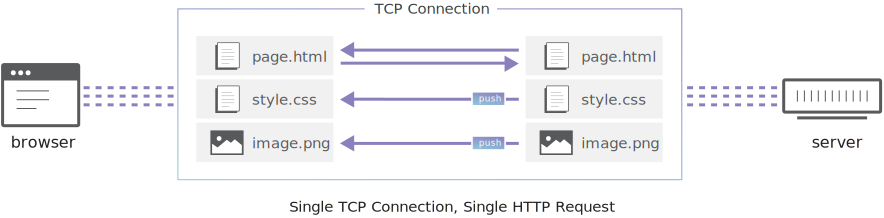
\includegraphics[width=1.55\textwidth]{./figures/http2_server_push.pdf}
%   \caption[][11em]{Schematische Darstellung der Verarbeitung von HTTP/2 Server Push~\citep{vlad:2016}.}
%   \label{fig:schema_http2_server_push}
% \end{figure}
%
%
% Abbildung~\ref{fig:server_push_ohne} \&~\ref{fig:server_push_mit} zeigt die Browser-seitige Verarbeitung einer Demonstrationswebseite auf der neben der Hauptseite fünf Grafiken enthalten sind -- je einmal ohne Server Push (Abbildung~\ref{fig:server_push_ohne}) und einmal mit (Abbildung~\ref{fig:server_push_mit}).
% Mittels sog.\ Profiling Tools lässt sich der Geschwindigkeitszuwachs sehr schön visualisieren und benchmarken.
%
% \begin{figure}%
% 	\centering
%   \includegraphics[width=1.55\textwidth]{./figures/server_push_ohne.png}
%   \caption[][8em]{Verarbeitung einer Seite mit fünf Grafiken ohne Server Push~\citep{vlad:2016}.}
%   \label{fig:server_push_ohne}
% \end{figure}
% Wie in Abbildung~\ref{fig:server_push_ohne} zu sehen ist, initiiert der Browser im Anschluss an das Laden der Hauptseite einen weiteren Request für die fünf enthaltenen Grafiken. Nachdem der Server den erneuten Request verarbeitet hat werden diese anschließend an den Browser ausgeliefert und von diesem angezeigt.
%
% \begin{figure}%
% 	\centering
%   \includegraphics[width=1.55\textwidth]{./figures/server_push_mit.png}
%   \caption[][8em]{Verarbeitung der Beispielseite mit Server Push~\citep{vlad:2016}.}
%   \label{fig:server_push_mit}
% \end{figure}
%
% Mit aktiviertem Server Push werden die Grafiken noch während der Client-seitigen Verarbeitung der Seite automatisch durch den Server ausgeliefert; eine zusätzliche Anfrage ist demnach nicht notwendig und spart Zeit. Zusammen mit der automatischen Auslieferung der Grafiken schickt der Server ein \texttt{PUSH\_PROMISE} Frame\sidenote{Durch \textbf{Push Promisies} signalisiert der Server dem Browser einen \texttt{PUSH} von zu einer Seite gehörenden Ressourcen. Dieses Frame wird immer automatisch am Beginn eines \texttt{PUSH} gesendet.} an den Browser. Sobald der Browser diese benötigt bzw.\ verarbeiten kann gleicht er diese mit dem \texttt{PUSH\_PROMISE} Frame ab und kann diese sofort ohne einen weiteren Request nutzen.
%
%
% ---- START ----
%
% Der beispielhafte Ablauf aus Abbildung~\ref{fig:http2_nachrichtenaustausch} (vgl.~Kapitel~\ref{sub:semantik_und_bestandteile}) zeigt die simultane Übertragung von zwei Streams innerhalb einer TCP-Verbindung. Im dritten Frame versendet der Server einen \texttt{PUSH\_PROMISE}-Frame innerhalb des Streams mit der ID \texttt{41}. Das passiert, weil der Server den nächsten Request des Clients vorhersagt und daraufhin eine Response ankündigt. Im genannten Beispiel sieht der Server eine Anfrage für eine Datei \texttt{style.css} kommen und kündigt deren Übertragung an den Client mit einem \texttt{HEADERS}-Frame an, den er im neuen Stream mit der ID \texttt{42} versendet.
%
% Der Client kann nun zwei Dinge tun. Um die angebotene Datei zu akzeptieren, muss der Client aktiv nichts weiter tun. Nach dem \texttt{HEADERS}-Frame wird der Server im Stream \texttt{42} einen \texttt{DATA}-Frame mit besagter Datei versenden. So erhält der Client die Datei \texttt{style.css} ohne sie jemals aktiv angefordert zu haben.
%
% Alternativ kann der Client zu der Entscheidung kommen, dass er die Datei \texttt{style.css} nicht benötigt. In diesem Fall schließt der Client den Stream \texttt{42}, indem er einen \texttt{RST\_STREAM}-Frame an den Server schickt. Das Protokoll verbietet es dem Server, über Streams zu kommunizieren, für die der Client einen solchen Frame gesendet hat.
%
% Server-Push verringert die Latenz somit durch das Einsparen von Client-Requests. Dafür muss der Server jedoch in der Lage sein, die Anfragen des Clients zuverlässig zu antizipieren. Er muss den auszuliefernden Content und das Verhalten seiner Clients gut kennen, um nachfolgende Requests nach weiteren Inhalten vorherzusehen.
%
% Es ist Aufgabe der Webserver-Administratoren oder der Webentwickler, die Push-Funktionalität durch Konfiguration und Implementierung zu gewährleisten.
%
% ---- END ----
%
%
% \subsection{Browserunterstützung} % (fold)
% \label{sub:browserunterstutzung}
% Laut der Website ``Can I use''\sidenote{\url{https://caniuse.com/\#search=http\%2F2}} wird HTTP/2 bereits von 87,59\% der Internet Browser in Deutschland und 79,57\% der Browser weltweit unterstützt (Stand 2. März 2018).
% Mittlerweile unterstützen auch die meisten mobilen Browser HTTP/2.
% Microsoft's Internet Explorer 11 unterstützt das Protokoll, jedoch nur unter Windows 10.
% Einschränkungen gibt es auch bei Firefox und Chrome, welche HTTP/2 nur unterstützen, falls der Server die TLS-Protokollerweiterung \textbf{Application-Layer Protocol Negotiation (ALPN)}\sidenote{\url{https://en.wikipedia.org/wiki/Application-Layer\_Protocol\_Negotiation}} unterstützt.
% Generell (mit Ausnahme des IE11) muss das TLS-Protokoll Server-seitig implementiert und unterstützt werden.
% Aufgrund der Abwärtskompatibilität werden Webseiten Webseiten trotzdem ohne Probleme übertragen, wenn auch nur über HTTP/1.1.
% Weitere Details finden sich auf den Seiten von ``Can I use''. % \url{https://caniuse.com/#search=http%2F2}.
%
% \begin{figure}%
% 	\centering
%   \includegraphics[width=1.55\textwidth]{./figures/http2_browser_support.png}
%   \caption[][26em]{Übersicht der Browserunterstützung von HTTP/2}
%   \label{fig:http2_browser_support}
% \end{figure}
%
%
%
%
%
%
%
%
%
%
% \section{Zusammenfassung} % (fold)
% \label{sec:zusammenfassung}
% Durch die Protokollversion HTTP/2 wird die Geschwindigkeit, Effizienz und Sicherheit der Datenübertragung verbessert. HTTP/1.1 verwendet zum Laden von unterschiedlichen Seitenelementen wie JS-, CSS- und Bilddateien mehrere TCP Verbindungen. Im Vergleich dazu werden bei http/2 mehrere Daten parallel über nur eine Verbindung übertragen, was die Ladezeiten deutlich beschleunigt. Die Technik, die hierfür verwendet wird, nennt sich Multiplexing. Auch die Art und Weise wie Header Daten übertragen werden, unterscheiden sich bei beiden Protokollen. Im Gegensatz zur HTTP 1.1 Verbindung, bei der die Daten unkomprimiert verschickt werden, übertragt HTTP/2 die Informationen komprimiert im Binärcode. Dadurch soll zusätzlich die Verarbeitung der Daten beschleunigt werden. Weitere Vorteile von HTTP/2 im Vergleich zu HTTP/1.1 sind die Priorisierung von Datenpaketen, der Server Push und der Wegfall von Head-of-Line-Blocking. Datenpakete werden nach Wichtigkeit sortiert und in entsprechender Reihenfolge übermittelt, wodurch zuerst die Dateien an den Browser übermittelt werden, die für einen schnellen Seitenaufbau wichtig sind. Über den Server Push können JSS, CSS und andere Dateiformate dabei ohne vorherige Anfrage des Clients übermittelt werden. Durch den Wegfall von Head-of-Line-Blocking kann es in HTTP/2 nicht mehr zu dem Problem kommen, dass durch die Verzögerung bei der der Übertragung eines Datenpakets alle folgenden Datenpakete blockiert werden. Dieses Problem besteht bisher noch in HTTP/1.1.
%
% % section zusammenfassung (end)


\newpage
\bibliography{refs}
\bibliographystyle{plainnat} % SZA: was plainnat




\end{document}